\clearpage
\section{Frequency}
The frequency of a trigonometric function is defined as the reciprocal of its period. For example, if the period of a function is $2\pi$, it's frequency is $\frac{1}{2\pi}$. To generalize:
\begin{definition}
    The frequency of a trigonometric function is
    \[
        P^{-1} \text{ or } \frac{1}{P} \text{,}
    \]
    where $P$ is the period of the function.
\end{definition}
If the period of a function is how long it takes for it to complete one full cycle, the frequency of a function is how much of the cycle was reached in some interval (usually $1$ unit).

To demonstrate, I'll use the function $\cos(x)$. In the section on the period of sine and cosine, we learn that $\cos(x)$ has a period of $2\pi$. We take the reciprocal of this to find that its frequency is $\frac{1}{2\pi}$, which is approximately $0.159155$. This means that, after one radian, routhly $15.9155\%$ of the cycle is completed.

In other words, if you separated $\cos(x)$ in the interval $x \in [0, 2\pi]$ into subintervals that are $1$ unit long, you'd end up with $2\pi \approx 6.283185$ intervals. The below graph demonstrates this.
\begin{center}
    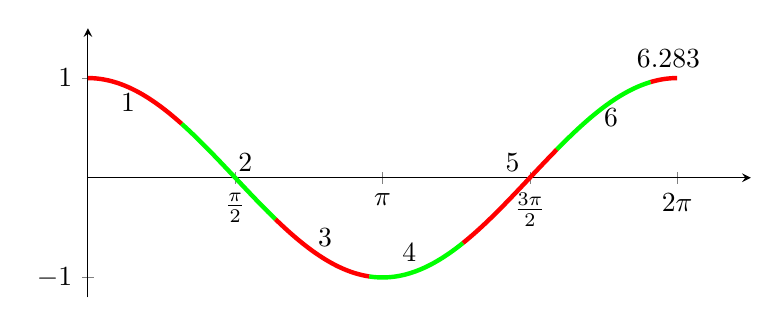
\begin{tikzpicture}
        \begin{axis}[%
            xmin = 0, xmax = (9 * pi) / 4,
            ymin = -1.2, ymax = 1.5,
            xtick = {
                0,
                pi / 2,
                pi,
                (3 * pi) / 2,
                2 * pi%
            },
            xticklabels = {
                $0$,
                $\frac{\pi}{2}$,
                $\pi$,
                $\frac{3\pi}{2}$,
                $2\pi$
            },
            width = 10cm, height = 5cm,
            trig format plots=rad,
            axis lines = center%
        ]
        \addplot[color = red, ultra thick, domain = 0:1, samples = 100] {cos(x)};
        \node[right] at (0.25, 0.75) {$1$};
        
        \addplot[color = green, ultra thick, domain = 1:2, samples = 100] {cos(x)};
        \node[right] at (1.5, 0.15) {$2$};

        \addplot[color = red, ultra thick, domain = 2:3, samples = 100] {cos(x)};
        \node[right] at (2.35, -0.6) {$3$};

        \addplot[color = green, ultra thick, domain = 3:4, samples = 100] {cos(x)};
        \node[right] at (3.25, -0.75) {$4$};

        \addplot[color = red, ultra thick, domain = 4:5, samples = 100] {cos(x)};
        \node[right] at (4.35, 0.15) {$5$};

        \addplot[color = green, ultra thick, domain = 5:6, samples = 100] {cos(x)};
        \node[right] at (5.4, 0.6) {$6$};

        \addplot[color = red, ultra thick, domain = 6:{2 * pi}, samples = 100] {cos(x)};
        \node[right] at (5.75, 1.2) {$6.283$};
        \end{axis}
    \end{tikzpicture}
\end{center}
This idea can be extended to any period, hence the definition. Also, because of the direction relationship between the period and frequency of a trigonometric function, we can solve for one if we have the other.
\clearpage
In the example above, we used the period to find the frequency. However, if we have the frequency, we can find the period with a little algebra.
\[
    \text{If } F = \frac{1}{P}\text{, then } P = \frac{1}{F} \text{.}
\]
Try this for size:
\begin{problem}
    Given the the frequency of some trigonometric function $f$ is $0.384$, find the period $P$ of the function.
\end{problem}
\begin{solution}
    All we need to do to find the period is the take the reciprocal of this frequency. If $F = 0.384$, then
    \begin{align*}
        P = \frac{1}{0.384} = \frac{1000}{384} = \frac{125}{48} \approx 2.604167
    \end{align*}
\end{solution}
